%\documentclass[handout]{beamer}
\documentclass{beamer}

%-----------------------------
%           PACKAGES

\usepackage[T1]{fontenc}
\usepackage[utf8]{inputenc}
\usepackage{eulervm}
\usepackage[scaled]{helvet}
\usepackage{graphicx}
\usepackage{amsmath,amsfonts,amssymb}
\usepackage{tikz}

\usetikzlibrary{positioning,arrows}
\usetikzlibrary{decorations.pathmorphing}
\usetikzlibrary{decorations.markings}

\usetheme{Warsaw}
\usefonttheme[onlymath]{serif}
\usecolortheme{Ben}
%\usecolortheme{fly}

\newcommand{\grille}{
    \begin{tikzpicture}[overlay,remember picture]
        \begin{scope}[shift={(current page.south west)}]
            \draw[gray!50] (0,0) grid[step=2mm] (current page.north east);
            \draw[red!50] (0,0) grid[step=1cm] (current page.north east);
            \draw (0.2,1) node {1};
            \draw (0.2,2) node {2};
            \draw (0.2,3) node {3};
            \draw (0.2,4) node {4};
            \draw (0.2,5) node {5};
            \draw (0.2,6) node {6};
            \draw (0.2,7) node {7};
            \draw (0.2,8) node {8};
            \draw (0.2,9) node {9};
            \draw (1,0.5) node {1};
            \draw (2,0.5) node {2};
            \draw (3,0.5) node {3};
            \draw (4,0.5) node {4};
            \draw (5,0.5) node {5};
            \draw (6,0.5) node {6};
            \draw (7,0.5) node {7};
            \draw (8,0.5) node {8};
            \draw (9,0.5) node {9};
            \draw (10,0.5) node {10};
            \draw (11,0.5) node {11};
            \draw (12,0.5) node {12};
        \end{scope}
    \end{tikzpicture}
}
\newcommand{\degres}{\ensuremath{^\circ}}
\title[Ph. D. defense]{Développement d'une échelle double face pour la trajectométrie en physique des hautes énergies.}
\subtitle{Ph. D. defense}
\institute{DESY}
\author[Benjamin BOITRELLE]{Benjamin BOITRELLE  \\ Supervisors: Jérôme Baudot, Ingrid Maria Gregor} %\\ On behalf of the PLUME Collaboration
\date{February 13, 2017}
\defbeamertemplate*{footline}{shadow theme}
%\titlegraphic{
\includegraphics[scale = 0.08]{Pictures/DESY-Logo.png}}
{%
    \leavevmode%
    \hbox{\begin{beamercolorbox}[wd=.5\paperwidth,ht=2.5ex,dp=1.125ex,leftskip=.3cm plus1fil,rightskip=.3cm]{author in head/foot}%
            \usebeamerfont{author in head/foot}\insertframenumber\,/\,\inserttotalframenumber\hfill\insertshortauthor
        \end{beamercolorbox}%
        \begin{beamercolorbox}[wd=.5\paperwidth,ht=2.5ex,dp=1.125ex,leftskip=.3cm,rightskip=.3cm plus1fil]{title in head/foot}%
            \usebeamerfont{title in head/foot}\insertshorttitle%
    \end{beamercolorbox}}%
    \vskip0pt%
}

%-------------
%
% INTRODUCTION:
%   - What is the SM?
%   - Higgs boson
%   - ILC and ILD
%
% WORK:
%   - PLUME and CMOS
%   - Impact parameter
% 
% CONCLUSION AND OUTLOOK

\begin{document}

  \begin{frame}[plain]
    \maketitle
    \begin{columns}[t]
        \begin{column}{2cm}
            
\includegraphics[width = 2cm, height = 2cm]{Pictures/DESY-Logo.png}
        \end{column}

        \begin{column}{3cm}
            
\includegraphics[width = 3cm, height = 2cm]{Pictures/logo_IPHC_10cm.png}
        \end{column}
        \begin{column}{3cm}
            
\includegraphics[width = 3cm, height = 2cm]{Pictures/logo_uni_stra.jpg}
        \end{column}        
        \begin{column}{3cm}
            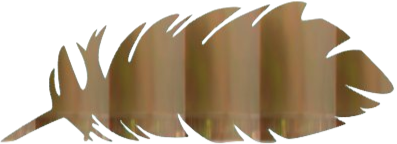
\includegraphics[width = 3cm, height = 1.5cm]{Pictures/logo_plume.png}
        \end{column}
    \end{columns}

  \end{frame}

  \begin{frame}[plain]
    \frametitle{Outlines}

    \tableofcontents
  \end{frame}

  \section{Introduction}
    \subsection{Standard Model}
    \subsection{Higgs Boson}
    \subsection{ILC and ILD}
%-------------------------------
%   Intro: ILC 
%-------------------------------

  \begin{frame}
    \frametitle{International Linear Collider}

    \vspace{-0.3cm}
    \begin{center}
      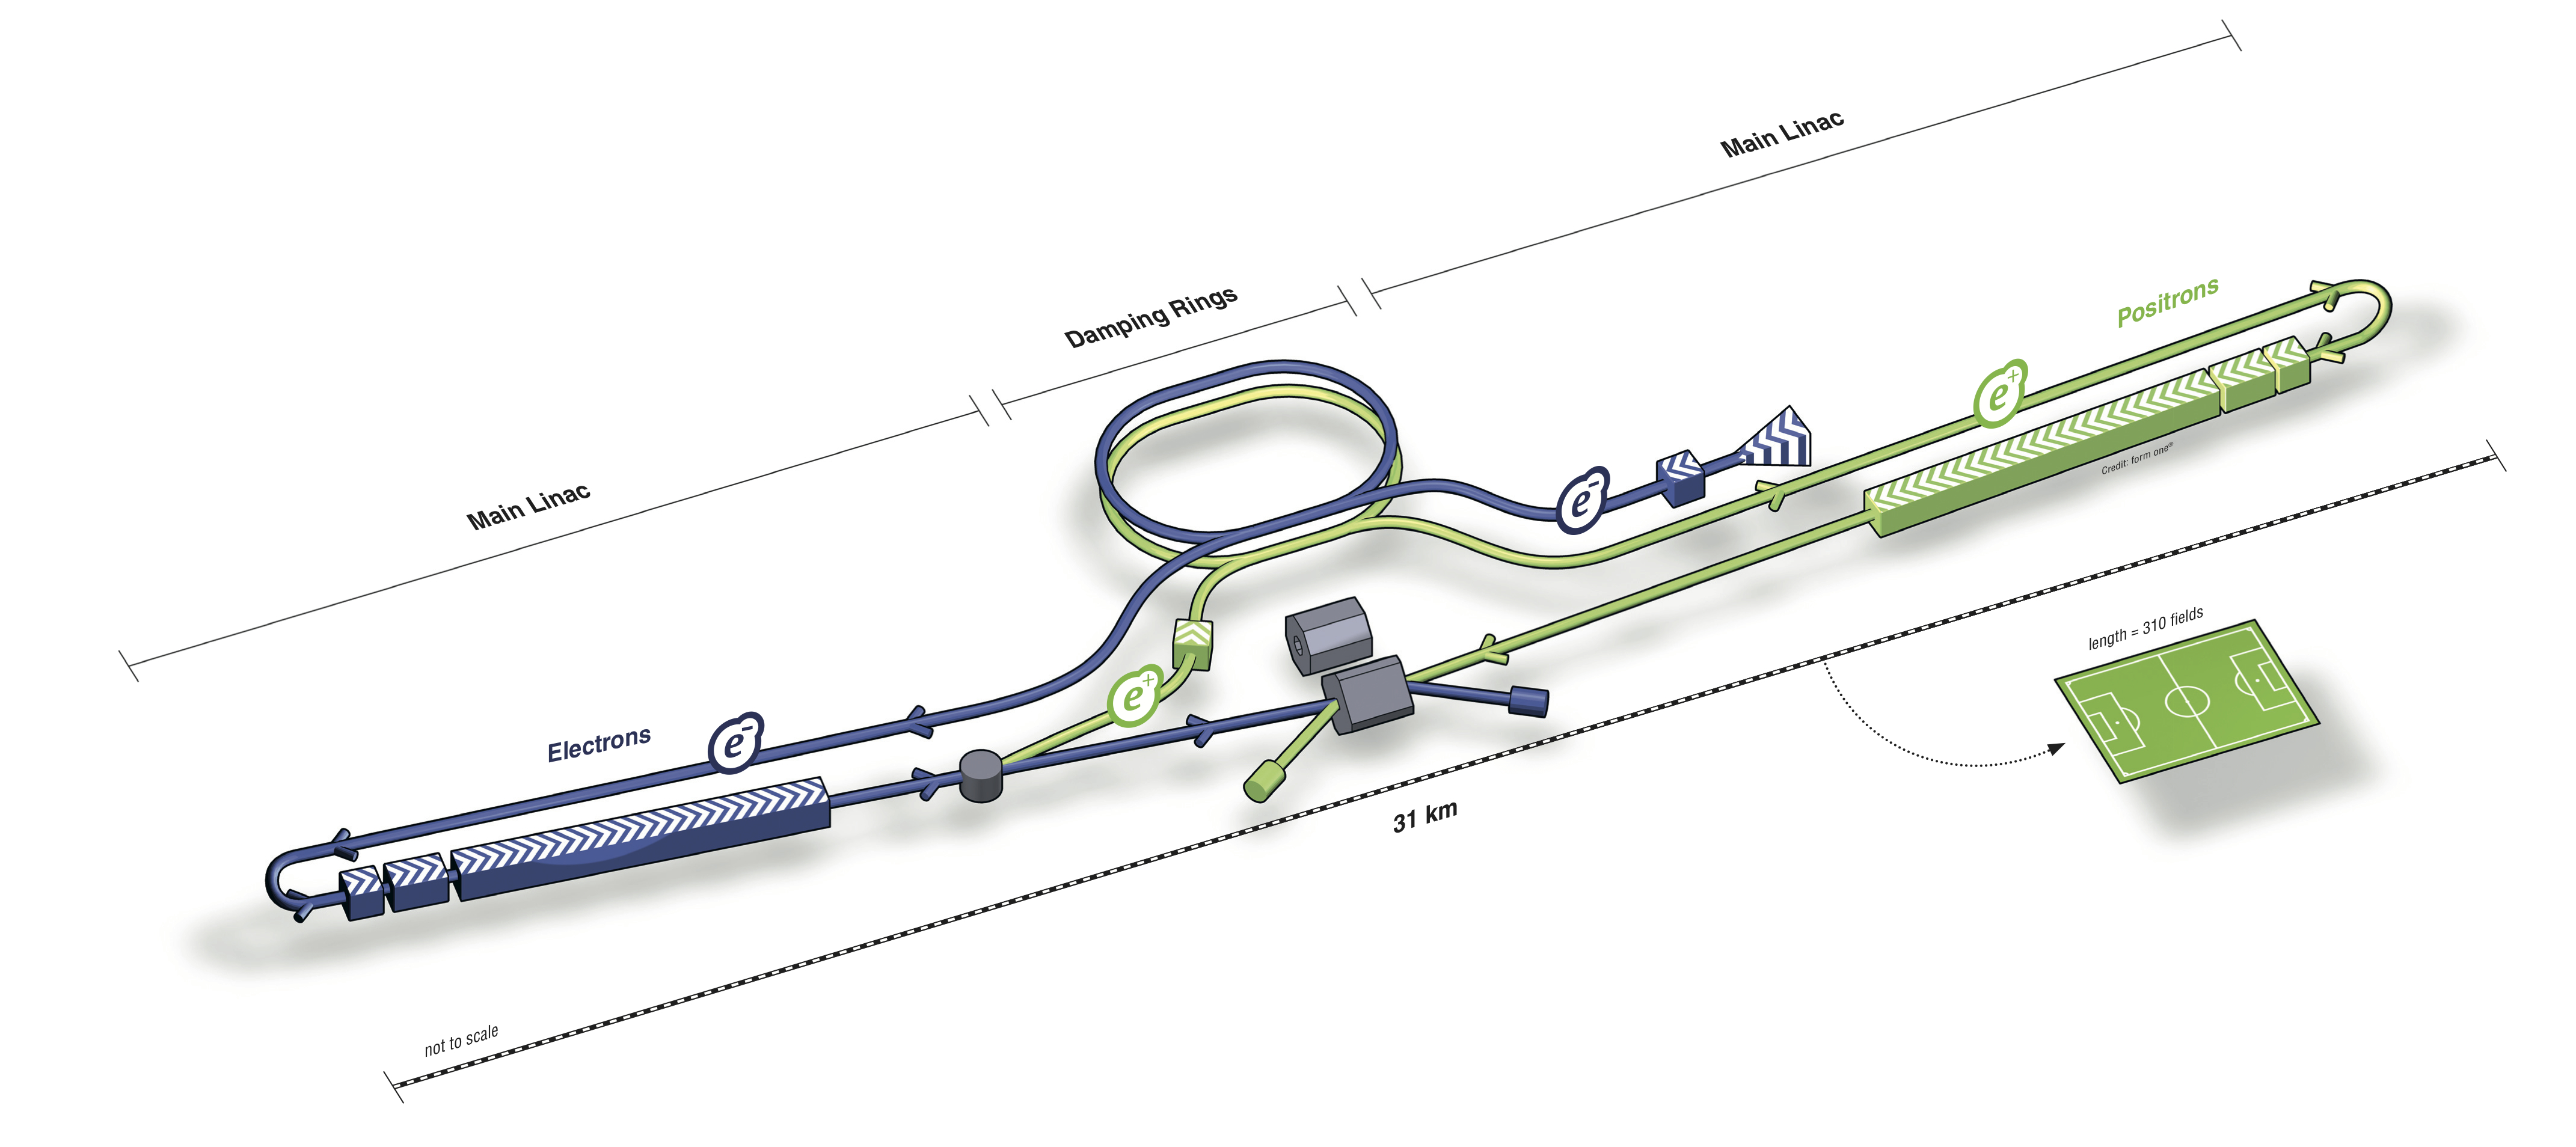
\includegraphics[width = 9 cm]{Pictures/ILC.png}
    \end{center}

    \vspace{-0.3cm}
    \begin{itemize}
      \item Future $\rm{e}^+\rm{e}^-$ linear collider at $\sqrt{s} = 250 - 500~\rm{GeV}$ \\ (upgrade up to $\sqrt{s} = 1~\rm{TeV}$)
      \item Polarised beam
      \item Luminosity $\simeq 2 \times 10^{34}~\rm{cm}^{-2}\rm{s}^{-1}$
      \item Candidate site: Kitakami in nothern Japan
      \item To study properties of the Higgs boson, top physics...
    \end{itemize}
  \end{frame}

%-------------------------------
%   INTRO: ILD VS SiD 
%-------------------------------

\subsection{The two experiments at the ILC}
\begin{frame}
  \frametitle{SiD and ILD}

  \vspace{-0.12cm}
  \begin{columns}[t]
    \begin{column}{5cm}
      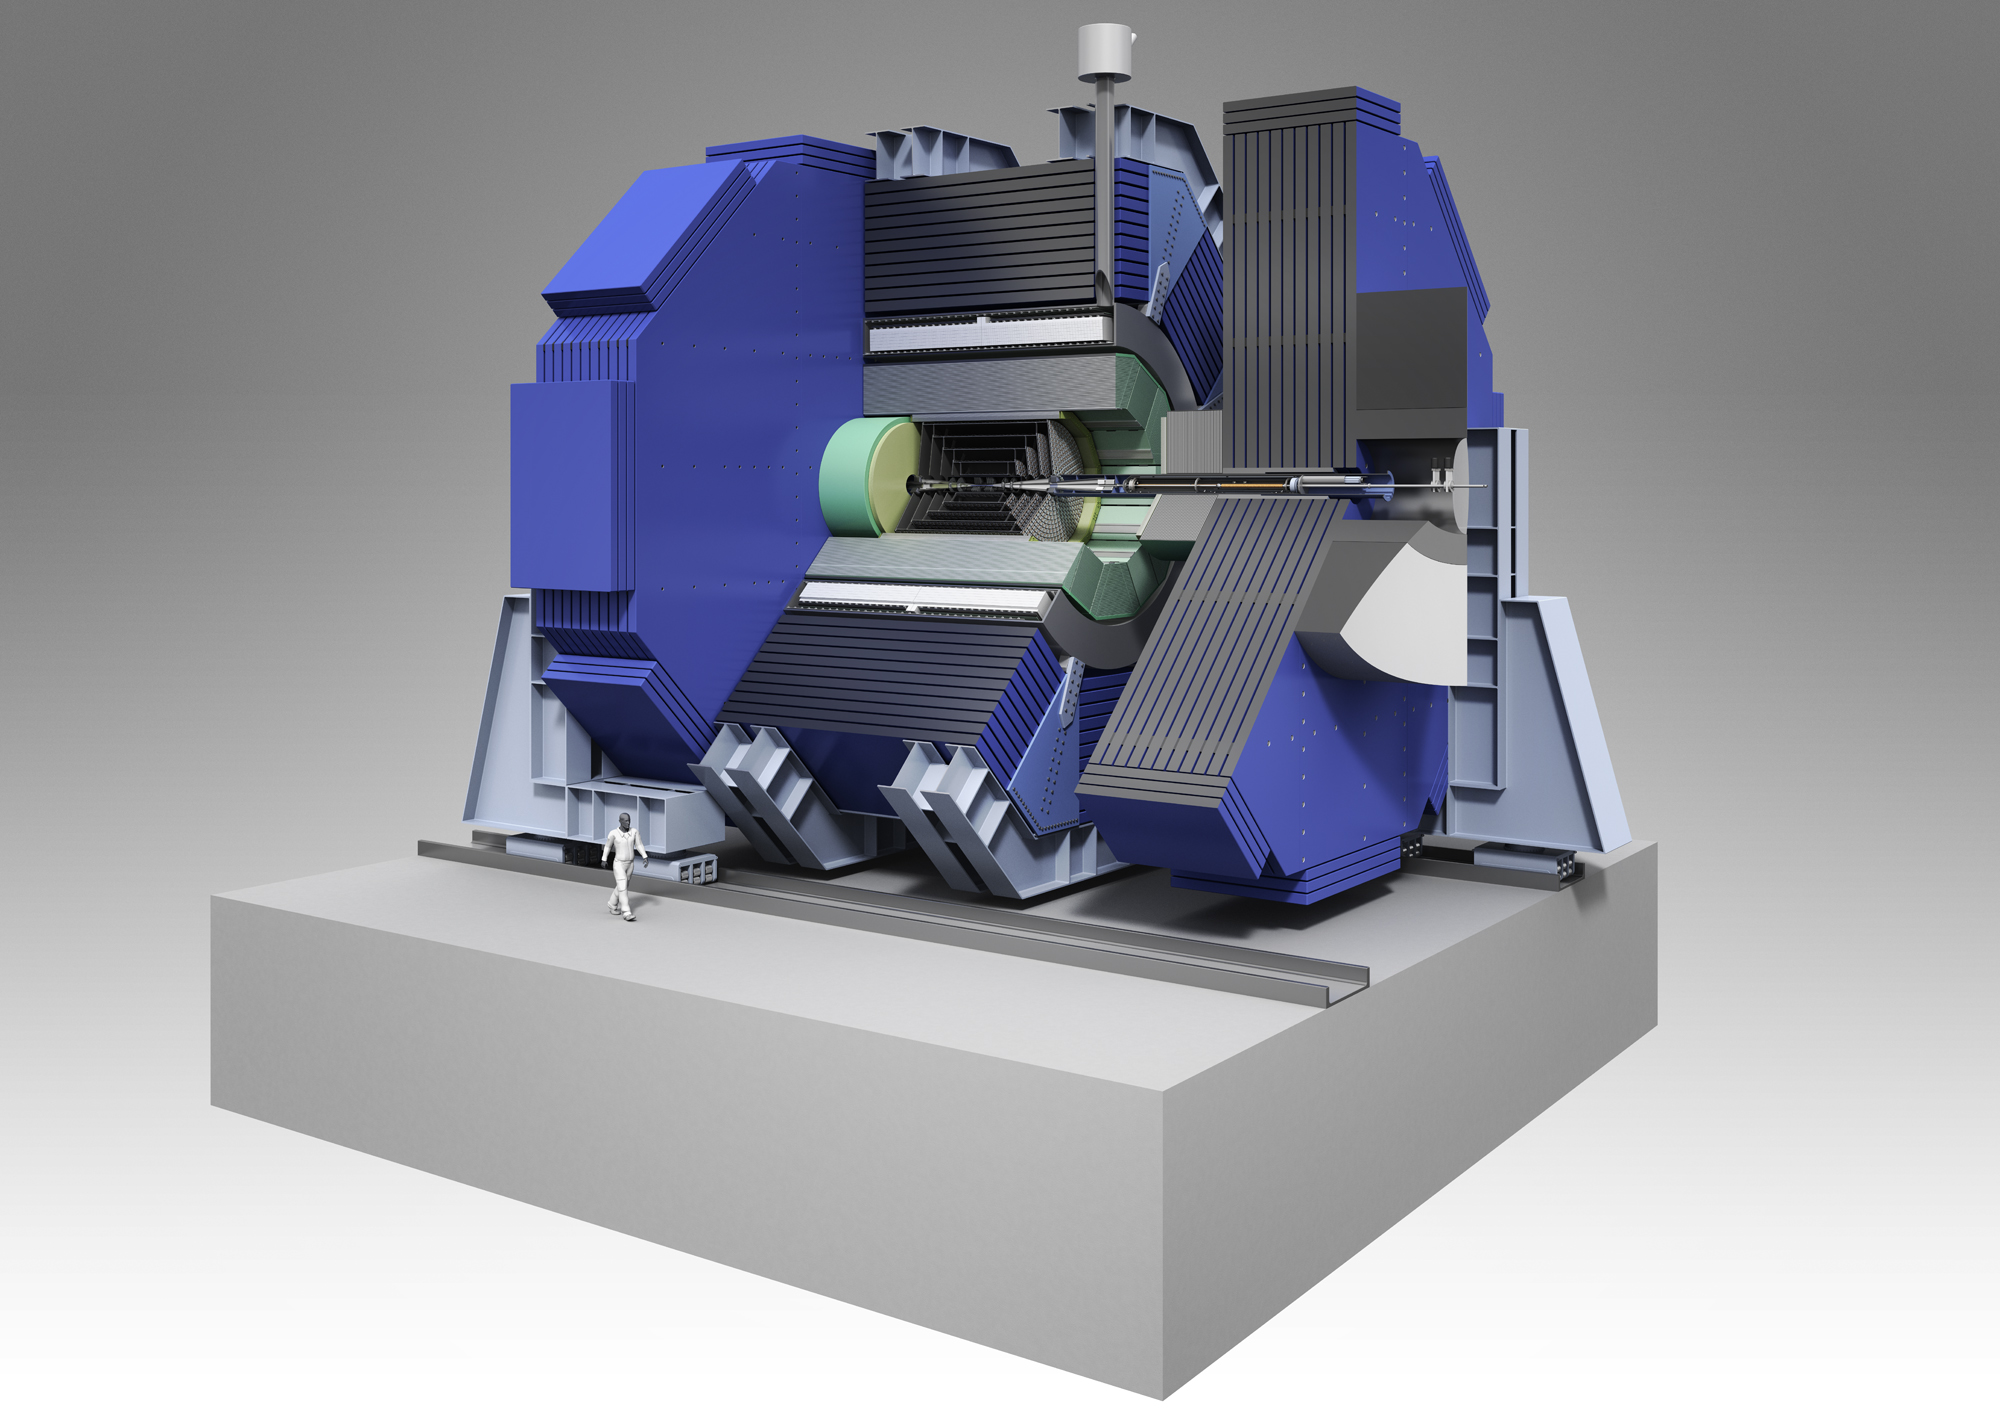
\includegraphics[width = 5cm, height = 2.9 cm]{Pictures/ILC_SiD.jpg}
      \vspace{-0.25cm}
      \begin{block}{Silicon Detector}
        \begin{itemize}
          \item Silicon tracking (radius = 1.2m)
          \item B$_{\rm{field}}$ = 5 T
        \end{itemize}
      \end{block}
    \end{column}

    \begin{column}{5cm}
      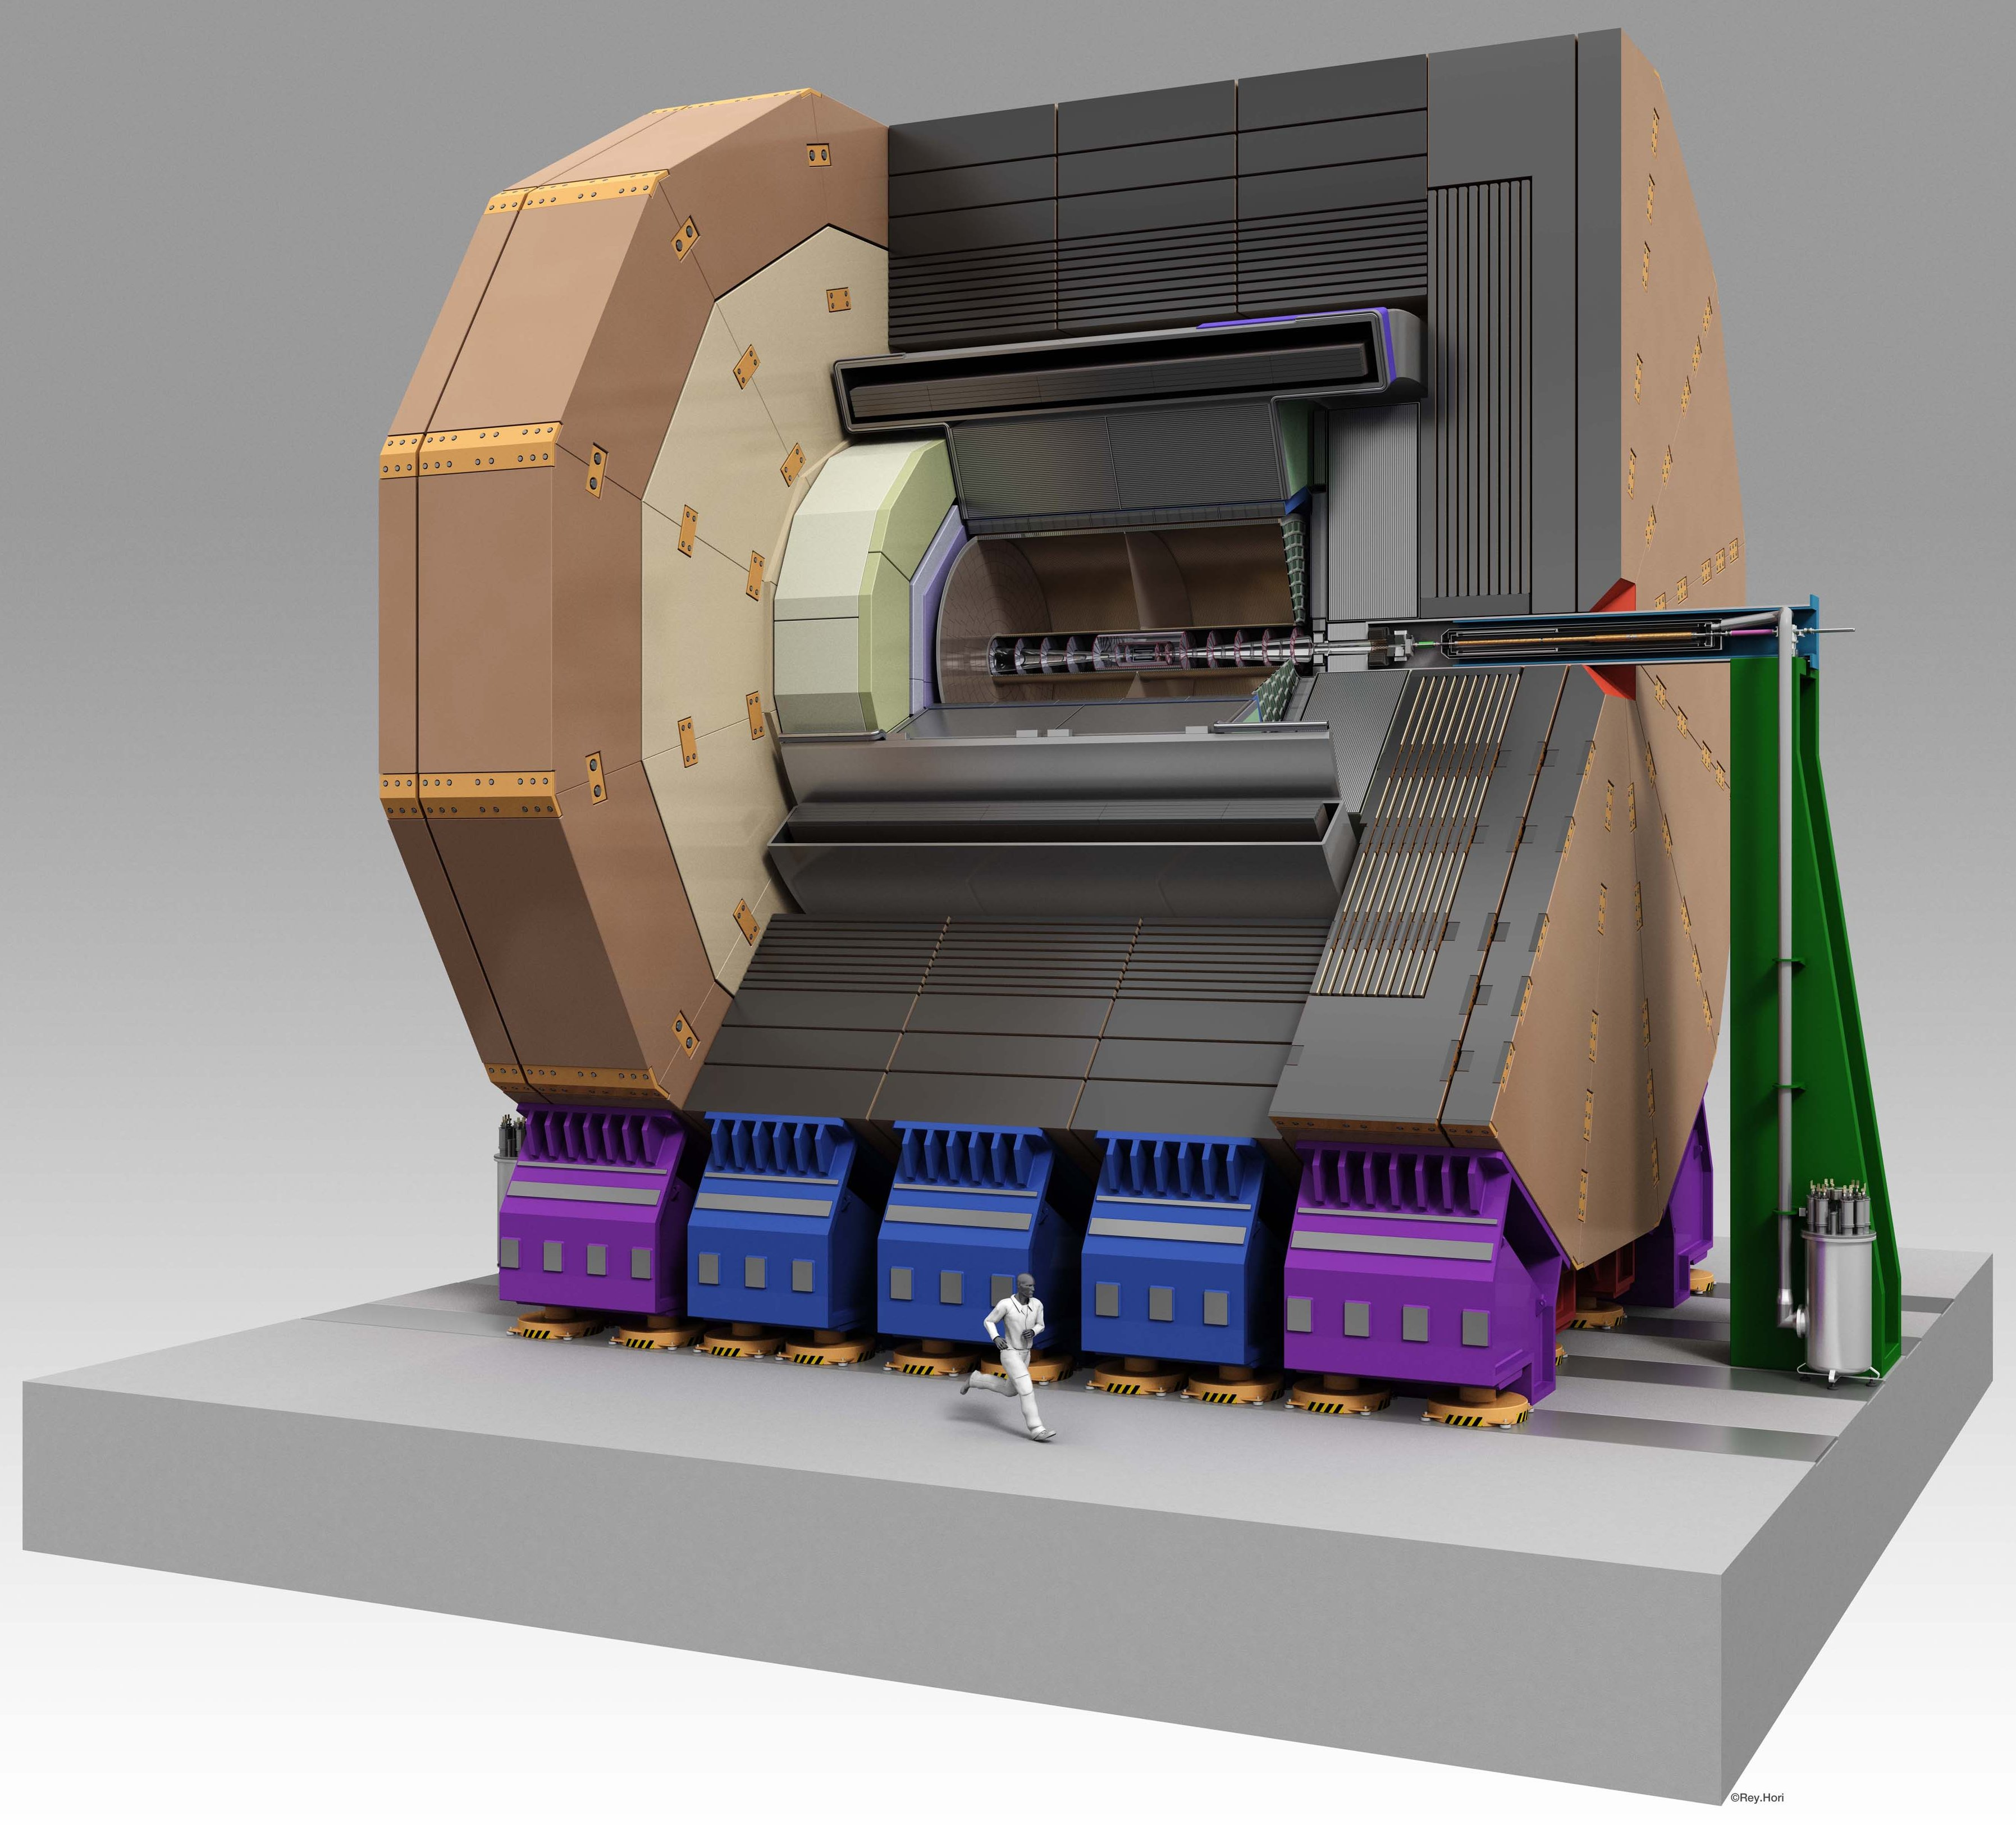
\includegraphics[width = 5cm, height = 2.9 cm]{Pictures/ILD_all_110826.jpg}
      \vspace{-0.25cm}
      \begin{block}{International Linear Detector}
        \begin{itemize}
          \item TPC + silicon envelope (radius = 1.8 m)
          \item B$_{\rm{field}}$ = 3.5 T
        \end{itemize}
      \end{block}
    \end{column}
  \end{columns}

  \vspace{-0.2cm}
  \begin{block}{Both detectors designed for Particle Flow Calorimetry}
      \begin{itemize}
          \item High granularity calorimeters (ECAL and HCAL) inside solenoid
              \vspace{-0.1cm}
          \item Low mass tracker to reduce interactions and conversions
      \end{itemize}
  \end{block}
\end{frame}

  %\section{Vertex detector}
  %  \subsection{CMOS sensors}
  %  \subsection{PLUME project}
  %  \subsection{Impact parameter}
    
  \section{Mechanical deformation}
    \subsection{TB-2011}
    \subsection{Spatial resolution}
    \subsection{Deformation}
  
  \section{Radiation length measurement}
    \subsection{TB-2016}
    \subsection{Theoretical estimation}
    \subsection{Results}
    
  \section{Conclusion and outlook} 

  \begin{frame}
    \begin{center}
      \huge
      \textbf{Thanks for your attention !!!}
    \end{center}
  \end{frame}
  %-------------------------------
%   BACK-UP
%-------------------------------

  \appendix
%-------------------------------
%   STOP FRAME COUNTING
%-------------------------------
  \newcounter{lastframe}
  \setcounter{lastframe}{\insertframenumber}
  %\setbeamertemplate{footline}[default]  % vide

%-------------------------------
%   BACK-UP: SUZE
%-------------------------------

  \begin{frame}[plain, label=suze]
    \frametitle{Zero Suppression logic (SUZE)}

    \vspace{-0.4cm}
    \begin{center}
        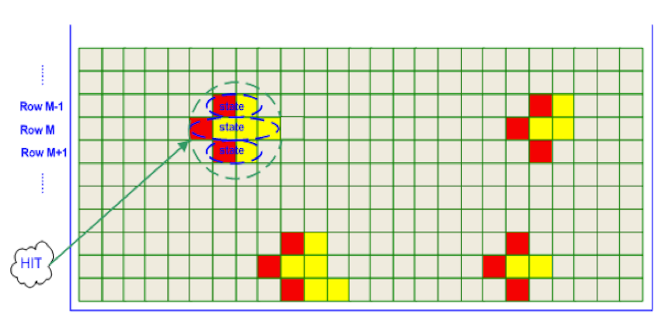
\includegraphics[width = 7 cm]{Pictures/suze_hitDetection.png}

        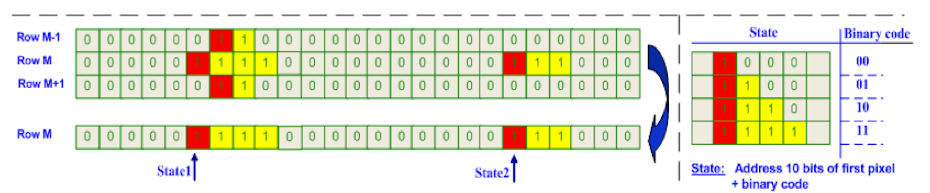
\includegraphics[width = 7cm]{Pictures/suze_hit2.png}
    \end{center}

    \vspace{-0.3cm}
    \scriptsize

    SUZE logic split in 3 blocks:
    \begin{itemize}
        \item \textbf{Sparse Data Scan (SDS)} Hit detection per line and data encoding, until 6 states consecutive pixels (1 to 4 pixels) per block of 64 columns;
        \item \textbf{Multiplexing Logic (Mux)} giving up to 9 states;
        \item \textbf{Memory storage} 2 blocks to store the states of the full frame, switching to avoid dead time (during one acquire states of event N, the other one transfer the information of frame N-1).
    \end{itemize}
    %\grille

  \end{frame}

%-------------------------------
%   BACK-UP: Spatial resolution VS pitch
%-------------------------------

  \begin{frame}[plain]
    \frametitle{Spatial resolution for different pitch (IPHC-Strasbourg)}

    \vspace{-0.3cm}
    \begin{center}
        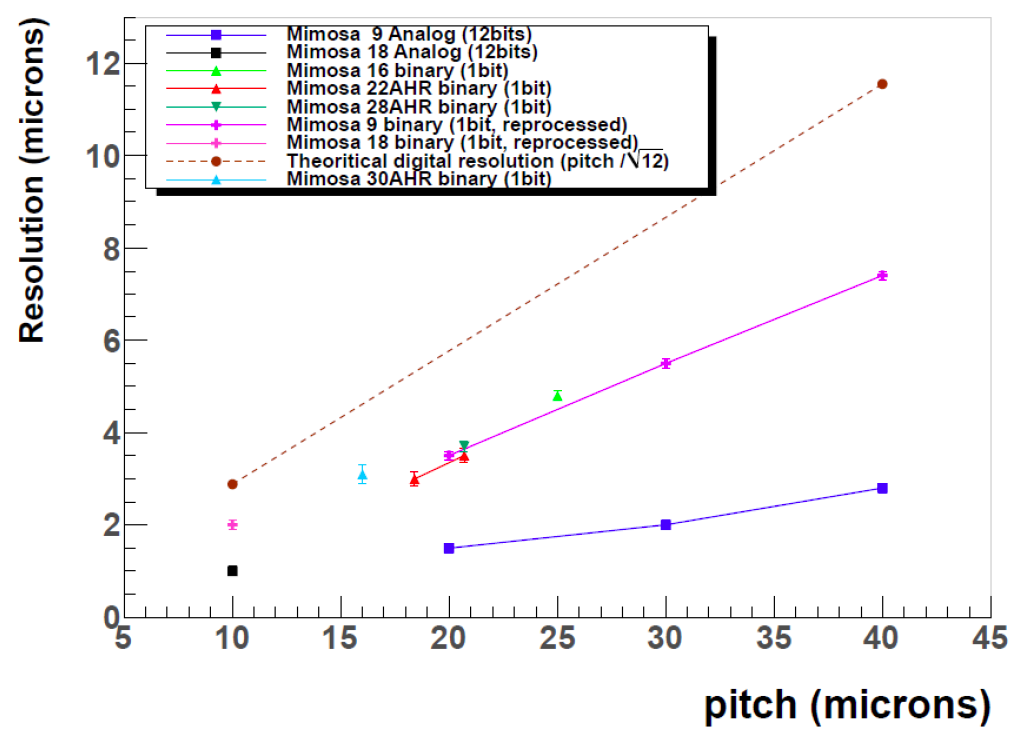
\includegraphics[width = 10cm]{Pictures/resolution_pitch_10to40_withBinary.png}
    \end{center}
  \end{frame}

%-------------------------------
%   BACK-UP: Physics
%-------------------------------

  \begin{frame}[plain]
    \frametitle{Higgs Strahlung kinematics}

    \[ E_H = \frac{s - \rm{M}_Z^2 + \rm{M}_H^2}{2\sqrt{s}} \]
    \[ E_Z = \frac{s - \rm{M}_H^2 + \rm{M}_Z^2}{2\sqrt{s}} \]
    \[ | \overrightarrow{p_H} | = | \overrightarrow{p_Z} | = \frac{\sqrt{\left[ s - (\rm{M}_H + \rm{M}_Z)^2 \right] \cdot \left[s - (\rm{M}_H - \rm{M}_Z)^2 \right]}}{2\sqrt{s}} \]

    If $\rm{M}_H = 125~\rm{GeV}$, $\rm{M}_Z = 91.2~\rm{GeV}$ and $\sqrt{s} = 350~\rm{GeV}$, then:
    \[ E_H \simeq 185.4~\rm{GeV} \]
    \[ E_Z \simeq 164.6~\rm{GeV} \]
    \[  | \overrightarrow{p_H} | = | \overrightarrow{p_Z} | \simeq 68.5~\rm{GeV}\]

  \end{frame}

%-------------------------------
%   BACK-UP: ILC-ILD
%-------------------------------
  \begin{frame}[plain]
    \frametitle{Detector performances}

    \begin{block}{Vertexing}
      \[ \sigma_{IP} \ = \ 5 \oplus \frac{10}{p\sin^{3/2}\theta} (\mu\rm{m})\]
    \end{block}

    \begin{block}{Tracking}
      \[ \sigma (1/p) \ = \ 2x10^{-5} (\rm{GeV}^{-1})\]
    \end{block}
      
    \begin{block}{Jet ernergy}
      \[\sigma_E / E \ = \ 0.3/\sqrt{\rm{E(GeV)}}\]
    \end{block}

  \end{frame}

%-------------------------------
%   BACK-UP: PFA
%-------------------------------
  \begin{frame}[plain]
    \frametitle{Particle Flow Algorithm}

    \begin{itemize}
      \item Typical jet:
        \begin{itemize}
          \item Charged hadrons $\simeq~60~\%$
          \item Photons $\simeq~30~\%$
          \item Neutral $\simeq~10~\%$
        \end{itemize}
      \item Standard approch
        \begin{itemize}
          \item All jet components energy measured in ECAL/HCAL
          \item $E_{jet} = E_{ECAL} + E_{HCAL}$
        \end{itemize}
      \item Particle flow calorimetry
        \begin{itemize}
          \item Measurement of charged particles in tracker
          \item Measurement of photon in ECAL
          \item Measurement of hadrons in HCAL
          \item $E_{jet} = E_{Track} + E_{\gamma} + E_n$
        \end{itemize}
    \end{itemize}
  \end{frame}
\end{document}
